\documentclass{article}
\usepackage{enumitem}
\usepackage{fancyhdr}
\usepackage[a4paper, left=1in, right=1in, top=1in, bottom=1in]{geometry}
\usepackage{amsfonts}
\usepackage{amsmath}
\usepackage[many]{tcolorbox}
\usepackage{xcolor}
\usepackage{cancel}
\usepackage{siunitx}
\tcbuselibrary{skins}

\pagestyle{fancy}
\cfoot{}
\lhead{}

\definecolor{chinayellow}{rgb}{0.82, 0.18, 0.6}
\definecolor{chinared}{rgb}{0.94, 0.82, 0.44}

\chead{\Large\bf Number Theory HW \#10 - Primality Testing}
\lhead{Page \thepage}
\rhead{Sonit Sahoo}
\setlength{\headheight}{18.0pt}

\newcommand\tagit{\addtocounter{equation}{1}\tag{\theequation}}

\newtcbtheorem[]{problem}{Problem}{
    enhanced,
    colback = chinayellow!7,
    colbacktitle = chinayellow!7,
    coltitle = black,
    boxrule = 0pt,
    frame hidden,
    borderline west = {0.6mm}{0mm}{chinayellow},
    fonttitle = \bfseries,
    before skip = 3ex,
    after skip = 0pt,
    sharp corners,
    rounded corners = northeast,
    breakable
}{problem}
\newtcbtheorem[]{solution}{}{
    enhanced,
    colback = chinared!7,
    coltitle = chinared!7,
    boxrule = 0pt,
    frame hidden,
    borderline west = {0.6mm}{0mm}{chinared},
    before skip = 0pt,
    after skip = 3ex,
    sharp corners,
    fonttitle = \tiny,
    rounded corners = southeast,
    attach title to upper = {},
    title after break = {},
    title = {},
    breakable
}{solution}

\begin{document}

\begin{problem}{}{}
    Evaluate $\int\int_{\mathcal{R}} x-3y dA$ where $\mathcal{R}$ is region between $(0,0)$, $(2,1)$, and $(1,2)$. Use transformation $x=2u+v$ and $y=u+2v$.
    \begin{center}
    \begin{tikzpicture}[scale=2]
        \draw[->] (-0.5, 0) -- (2.5, 0) node[right] {$x$};
        \draw[->] (0, -0.5) -- (0, 2.5) node[above] {$y$};
        
        \filldraw[black] (0, 0) circle (1pt) node[below left] {$(0,0)$};
        \filldraw[black] (2, 1) circle (1pt) node[below right] {$(2,1)$};
        \filldraw[black] (1, 2) circle (1pt) node[above right] {$(1,2)$};
        
        \fill[blue!20, opacity=0.5] (0, 0) -- (2, 1) -- (1, 2) -- cycle;
        \draw[thick] (0, 0) -- (2, 1) -- (1, 2) -- cycle;
    \end{tikzpicture}
    \end{center}
\end{problem}
\begin{solution}{}{}
    \begin{align*}
        u&=y-2v\\
        v&=x-2u\\
        u&=y-2(x-2u) \\
        -3u&=y-2x \\
        &=\frac{2}{3}x-\frac{1}{3}y \\
        v&=x-2\left(\frac{2}{3}x-\frac{1}{3}y\right) \\
        &=-\frac{1}{3}x+\frac{2}{3}y
    \end{align*}
    We can then plug in the functions of all 3 sides, and find $(0,0)$, $(0,1)$, and $(1,0)$.
    \begin{center}
        \begin{tikzpicture}[scale=2]
            \draw[->] (-0.5, 0) -- (2.5, 0) node[right] {$u$};
            \draw[->] (0, -0.5) -- (0, 2.5) node[above] {$v$};
            
            \filldraw[black] (0, 0) circle (1pt) node[below left] {$(0,0)$};
            \filldraw[black] (1, 0) circle (1pt) node[below right] {$(1,0)$};
            \filldraw[black] (0, 1) circle (1pt) node[above right] {$(0,1)$};
            
            \fill[orange!20, opacity=0.5] (0, 0) -- (1, 0) -- (0, 1) -- cycle;
            \draw[thick] (0, 0) -- (1, 0) -- (0, 1) -- cycle;
        \end{tikzpicture}
        \end{center}
        This is a type 3 region!
        \begin{align*}
            \int\int_{\mathcal{R}} x-3y dA&=\int\int_{\mathcal{R}}((2u+v)-3(u+2v))\cdot\begin{vmatrix}
                \frac{\partial x}{\partial u} & \frac{\partial y}{\partial u} \\
                \frac{\partial x}{\partial u} & \frac{\partial y}{\partial v}
                \end{vmatrix}dudv\\
                &=\int_0^1\int_{0}^{-x}(-u-5v)\cdot\begin{vmatrix}
                    2 & 1 \\
                    1 & 2
                \end{vmatrix}dudv\\
                &=\int_0^1\int_{0}^{-x}(-u-5v)\cdot3 dudv\\&=\int_0^1\int_{0}^{-x}(-3u-15v) dudv
        \end{align*}
\end{solution}

\end{document}